% IEEE standard conference template; to be used with:
%   spconf.sty  - LaTeX style file, and
%   IEEEbib.bst - IEEE bibliography style file.
% --------------------------------------------------------------------------

\documentclass[letterpaper]{article}
\usepackage{spconf,amsmath,amssymb,graphicx,amsthm,newlfont,program,caption,subcaption}

% Example definitions.
% --------------------
% nice symbols for real and complex numbers
%\newcommand{\R}[0]{\mathbb{R}}
%\newcommand{\C}[0]{\mathbb{C}}

% bold paragraph titles
\newcommand{\mypar}[1]{{\bf #1.}}

\theoremstyle{definition}
\newtheorem{observation}{Observation}

\newtheorem{algorithm}{Algorithm}

% Title.
% ------
\title{A Descriptive Title, not too general, not too long}
%
% Single address.
% ---------------
\name{Markus P\"uschel\thanks{The author thanks Jelena Kovacevic. This paper
is a modified version of the template she used in her class.}} 
\address{Department of Computer Science\\ ETH Z\"urich\\Z\"urich, Switzerland}

% For example:
% ------------
%\address{School\\
%		 Department\\
%		 Address}
%
% Two addresses (uncomment and modify for two-address case).
% ----------------------------------------------------------
%\twoauthors
%  {A. Author-one, B. Author-two\sthanks{Thanks to XYZ agency for funding.}}
%		 {School A-B\\
%		 Department A-B\\
%		 Address A-B}
%  {C. Author-three, D. Author-four\sthanks{The fourth author performed the work
%		 while at ...}}
%		 {School C-D\\
%		 Department C-D\\
%		 Address C-D}
%

\begin{document}
%\ninept
%
\maketitle
%

\clearpage
\iffalse

The hard page limit is 6 pages in this style. Do not reduce font size
or use other tricks to squeeze. This pdf is formatted in the American letter format, so the spacing may look a bit strange when printed out.

\begin{abstract}
Describe in concise words what you do, why you do it (not necessarily
in this order), and the main result.  The abstract has to be
self-contained and readable for a person in the general area. You
should write the abstract last.
\end{abstract}

\section{Introduction}\label{sec:intro}

Do not start the introduction with the abstract or a slightly modified
version. It follows a possible structure of the introduction. 
Note that the structure can be modified, but the
content should be the same. Introduction and abstract should fill at most the first page, better less.

\mypar{Motivation} The first task is to motivate what you do.  You can
start general and zoom in one the specific problem you consider.  In
the process you should have explained to the reader: what you are doing,
why you are doing, why it is important (order is usually reversed).

For example, if my result is the fastest sorting implementation ever, one
could roughly go as follows. First explain why sorting is important
(used everywhere with a few examples) and why performance matters (large datasets,
realtime). Then explain that fast implementations are very hard and
expensive to get (memory hierarchy, vector, parallel). 

Now you state what you do in this paper. In our example: 
presenting a sorting implementation that is
faster for some sizes as all the other ones.

\mypar{Related work} Next, you have to give a brief overview of
related work. For a report like this, anywhere between 2 and 8
references. Briefly explain what they do. In the end contrast to what
you do to make now precisely clear what your contribution is.

\section{Background: Whatever the Background is}\label{sec:background}

Give a short, self-contained summary of necessary
background information. For example, assume you present an
implementation of sorting algorithms. You could organize into sorting
definition, algorithms considered, and asymptotic runtime statements. The goal of the
background section is to make the paper self-contained for an audience
as large as possible. As in every section
you start with a very brief overview of the section. Here it could be as follows: In this section 
we formally define the sorting problem we consider and introduce the algorithms we use
including a cost analysis.

\mypar{Sorting}
Precisely define sorting problem you consider.

\mypar{Sorting algorithms}
Explain the algorithm you use including their costs.

As an aside, don't talk about "the complexity of the algorithm.'' It's incorrect,
problems have a complexity, not algorithms.

\fi


\section{Your Proposed Method}\label{sec:yourmethod}

The purpose of this section is to review a convex hull sequential algorithm for sorted input set and common tangent line algorithm. We also present parallel algorithms for computing a convex hull of a sorted set of points.

\subsection{Sequential algorithm}

\subsection{Common tangent line algorithm}

\subsection{Parallel algorithms}

Algorithms presented here enable computing the upper hull of the input set. 
Computing lower hull can be done in a similar way and for simplicity its description is omitted in this report. 
Therefore, in this section, whenever we write ''convex hull'' we are referring to the upper hull.
% TODO(matalek): should we maybe replace everywhere to upper hull?
However, our implementation computes the entire convex hull (upper and lower).  

\subsubsection{General scheme}
Let $k$ denote the number of processors available and $n$ - number of points in the input set.
Let $P = \{p_0, p_1, ..., p_{n-1} \}$ be the sorted (by $x$ coordinate) set of input points.
Finally, let $CH(S)$ denote the convex hull of $S$ set and $R=CH(S)$.
All presented here algorithms share common approach.

Firstly, we divide the input set into $t$ equal sets based on the $x$ coordinate:
$$P_0 = \{p_0, p_1, ..., p_{\lceil{\frac{n}{k}}\rceil - 1}\}$$
$$P_1 = \{p_{\lceil{\frac{n}{k}}\rceil}, p_{\lceil{\frac{n}{k}}\rceil + 1}, ..., p_{\lceil{2 * \frac{n}{k}}\rceil - 1}\}$$
$$...$$
$$P_{k-1} = \{p_{(k-1)\lceil{\frac{n}{k}}\rceil}, p_{(k-1)\lceil{\frac{n}{k}}\rceil + 1}, ..., p_{n- 1} \}$$


Then, we execute sequential version of the convex hull algorithm (Andrew's monotone chain) for each of these sets in parallel, using $t$ threads.
As a result we have convex hull for each of the sets:
$$C_i = CH(P_i) \textrm{\;\;\; for \;} i \in \{0, 1, ..., k - 1\}$$

For the next step we need the following simple observation:
\begin{observation}
If $p \in P_i$ for some $i \in \{0, 1, ..., k - 1\}$, but $p \notin C_i$, then $p \notin R$.
\end{observation}

The immediate conclusion follows:
\begin{observation}
$$C = CH(P_0 \cup P_1 \cup ... \cup P_{k - 1})$$
\end{observation}

This observation enables us to perform the last step of the algorithm.
It consists of merging partial convex hulls $C_0, C_1, ..., C_{k - 1}$ into one convex hull $R$.
This is the step, where our algorithms differ.
Each of the algorithm presents different ways of merging partial convex hulls.
All of them are, however, based on the common tangent line algorithm.

\subsubsection{Naive Parallel algorithm}

So called Naive Parallel algorithm is based on merging two convex hulls into one convex hull. 
Let $A$ and $B$ be two convex hulls so that for every $p \in A, q \in B$ we have $p.x < q.x$, where $\_.x$ denotes the $x$ coordinate of the given point.
Further, let $p_0, p_1, ..., p_{n-1}$ be the points of $A$ (sorted by $x$ coordinate) and similarly $q_0, q_1, ... q_{m-1}$ be the points of $B$.
Let $p_i \in A$ and $q_j \in B$ be such points that $\overline{p_iq_j}$ is a common tangent line for $A$ and $B$.
Then we know that points $p_{i+1}, p_{i + 2}, ..., p_{n - 1}$ and $q_{j + 1}, q_{j + 2}, ..., q_{m - 1}$ are not going to be in the resulting convex hull.
Therefore, we have:
$$CH(A \cup B) = \{ p_0, p_1, ..., p_{i - 1}, p_i, q_j, q_{j + 1}, ..., q_{m - 1} \}$$
For performing this merge we can use array-like data structure.
The time complexity of this is equal to $O(n + m)$.
% TODO(matalek): is it true? check with common tangent line complexity

Using this merge algorithm we can perform computing the convex hull of the entire set in the form of the tree. 
We assume that number of processors $k$ is the power of 2. 
Our algorithm consists of $\log k$ steps.
We start with $C_0, C_1, ..., C_{k-1}$ convex hulls.
In each step we are merging convex hull which were pairs of resulting convex hulls from the previous step. 
If $I_0, I_1, ..., I_{2l - 1}$ is an input for the step, then we compute the output: $O_0, O_1, ..., O_{l - 1}$ using $l$ processors. 
$i$-th processor computes $O_i = CH(I_{2i} \cup I_{2i+1})$ using merge algorithm presented above.
Example scheme for 4 processors is presented on figure \ref{fig:naive-parallel-scheme}.
Pseudocode for this algorithm is presented as algorithm \ref{alg:naive-parallel}.

% TODO(matalek): think if we should put it without page break.
\begin{algorithm}
\label{alg:naive-parallel}
\begin{program}
\mbox{A fast exponentiation procedure:}
\BEGIN \\ %
  level := k / 2;
  partial\_results := array(2 * k);
  \FOR i := 0 \TO level \STEP 1 \textrm{\bf{\;in parallel}} \DO
    partial\_results[k + i] := 
    \;\;\;\; sequential\_algorithm(input, i)
  \OD
  \WHILE level > 0 \DO
    \FOR i := 0 \TO level \STEP 1 \textrm{\bf{\;in parallel}} \DO
      pos = level + i;
      partial\_results[pos] := merge(
      \;\;\;\; partial\_results[2*pos],
      \;\;\;\; partial\_results[2 * pos + 1])
    \OD
    level /= 2;
  \OD
  print(partial\_results(1));

\END
\end{program}
\end{algorithm}

\begin{figure}\centering
  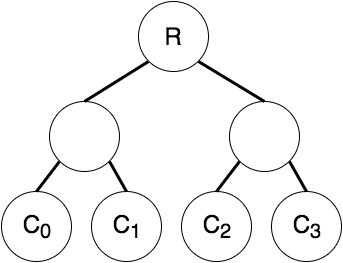
\includegraphics[scale=0.5]{img/naive-parallel}
  \caption{Scheme of merging convex hulls for $k=4$}
  \label{fig:naive-parallel-scheme}
\end{figure}

The time complexity of this algorithm depends on the size of the intermediates convex hulls.
In the worst case scenario size of the convex hull will be linear to the size of the input.
Then, time complexity of the algorithm can be estimated as:
$$O(\frac{n}{k}) + O(2\frac{n}{k}) + O(4\frac{n}{k}) + ... + O(k\frac{n}{k}) = O(n)$$
We can see that asymptotically this algorithm in the worst case scenario does not provide any speedup with more threads.
However, these calculations do not take into the account that calculating initial convex hull is connected with bigger constant than performing merging steps. 
% TODO(matalek): maybe more explanation

\subsubsection{Simple Parallel algorithm}

This algorithm was originally presented in \cite{SimpleParallel}.
It is based on computing what part of $C_i$ is also a part of $R$.
The computations are based on the following observation:
\begin{observation}
Let $P_i = \{q_0, q_1, ..., q_{l-1} \},$ where  $q_{j_1}.x < q_{j_2}.x$ for $0 \leq j_1 < j_2 < l$. 
We have, that for every $0 \leq j_1 < j_2 < j_3 < l$, if $q_{j_1}, q_{j_3} \in C_i$, then $q_{j_2} \in C_i$.
% TODO(matalek): do we need proof for it?
\end{observation}
We will call a point $p$ {\it\bf taken} if and only if $p \in P_i \land p \in C_i$ for some $i$. 
The above observation means that taken points from one convex hull form an interval (with regards to their indices).

Computing these intervals can be done by computing common tangent line for each pair $C_i$ and $C_j$.
For these pairs we know how  to compute intervals of taken points (see previous section). 
For given $i$ we can then compute intersection of the intervals computed for $C_i$ and $C_j$ for every $i \neq j$.
Let $[j_1, j_2]$ be the interval of indices corresponding to the calculated intersection.
If $j_1 < j_2$ then this interval corresponds also to the interval of taken points.
However, when $j_1 = j_2$ there might be two possible cases.
They are illustrated on the figure \ref{fig:simple-parallel}.
In the first case we have that the appropriate point is taken, in the second one - it is not.
The difference between these cases is the angle that common tangents line are forming.
In the first case, when going from left to right the angle between two steepest common lines is less than $\pi$, in the second case it is greater or equal $\pi$.
This means, that in the algorithm we need to keep track also of the steepest common tangent lines and use this information for this special case.
Solution for this special case was not presented in $\cite{SimpleParallel}$ and is originally developed by us.
% TODO(matalek): is above correct?

\begin{figure}
\centering
\begin{subfigure}{.3\textwidth}
	\centering
	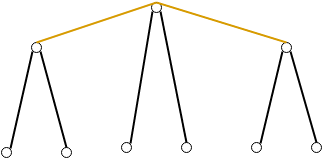
\includegraphics[width=\linewidth]{img/simple-parallel-taking}
	\caption{Point with index $j_1$ is taken}
\end{subfigure}
\begin{subfigure}{.3\textwidth}
	\centering
	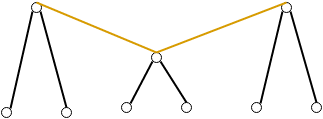
\includegraphics[width=\linewidth]{img/simple-parallel-not-taking}
	\caption{Point with index $j_1$ is not taken}
\end{subfigure}
\caption{Different possibilities for $j_1 = j_2$}
\label{fig:simple-parallel}
\end{figure}


These computations are done in parallel.
Processor $i$ computes all intervals for $C_i$ and $C_j$, where $j = 0, 1, ..., i -1, i+ 1, ..., k - 1$ and then computes their intersection.

The last steps consist of moving all taken points to one resulting array.
Firstly, we compute how many points from each convex hull $C_i$ are taken.
Let the result of this computation be: $l_1, l_2, ..., l_{k-1}$.
We can then compute starting positions in the resulting array for each taken points set from one convex hull.
Taken points from $C_i$ should be put at indices from $l_1 + l_2 + ... + l_{i-1}$ to $l_1 + l_2 + ... + l_{i-1} + l_i - 1$.
Calculating these indices can be done using parallel prefix computation.
We later copy taken points to the resulting array in parallel - each processor copies points from its own convex hull.


The time complexity for this algorithm, as shown in \cite{SimpleParallel}, is equal $O(\frac{n}{k} + k(\log \frac{n}{k})^2)$ and is optimal for $k \leq \frac{\sqrt{n}}{\log n}$.

\subsubsection{Hull Tree algorithm}

This algorithm was originally presented in \cite{HullTree}.

\iffalse
Now comes the ``beef'' of the report, where you explain what you
did. Again, organize it in paragraphs with titles. As in every section
you start with a very brief overview of the section.

In this section, structure is very important so one can follow the technical content.

Mention and cite any external resources that you used including libraries or other code.
\fi

\section{Experimental Results}\label{sec:exp}

Here you evaluate your work using experiments. You start again with a
very short summary of the section. The typical structure follows.

\mypar{Experimental setup} Specify the platform (processor, frequency, maybe OS, maybe cache sizes)
as well as the compiler, version, and flags used. If your work is about performance, 
I strongly recommend that you play with optimization flags and consider also icc for additional potential speedup.

Then explain what kind of benchmarks you ran. The idea is to give enough information so the experiments are reproducible by somebody else on his or her code.
For sorting you would talk about the input sizes. For a tool that performs NUMA optimization, you would specify the programs you ran.

\mypar{Results}
Next divide the experiments into classes, one paragraph for each. In each class of experiments you typically pursue one questions that then is answered by a suitable plot or plots. For example, first you may want to investigate the performance behavior with changing input size, then how your code compares to external benchmarks.

For some tips on benchmarking including how to create a decent viewgraph see pages 22--27 in \cite{Pueschel:10}.

{\bf Comments:}
\begin{itemize}
\item Create very readable, attractive plots (do 1 column, not 2 column plots
for this report) with readable font size. However, the font size should also not be too large; typically it is smaller than the text font size.
An example is in Fig.~\ref{fftperf} (of course you can have a different style).
\item Every plot answers a question. You state this question and extract the
answer from the plot in its discussion.
\item Every plot should be referenced and discussed.
\end{itemize}

\begin{figure}\centering
  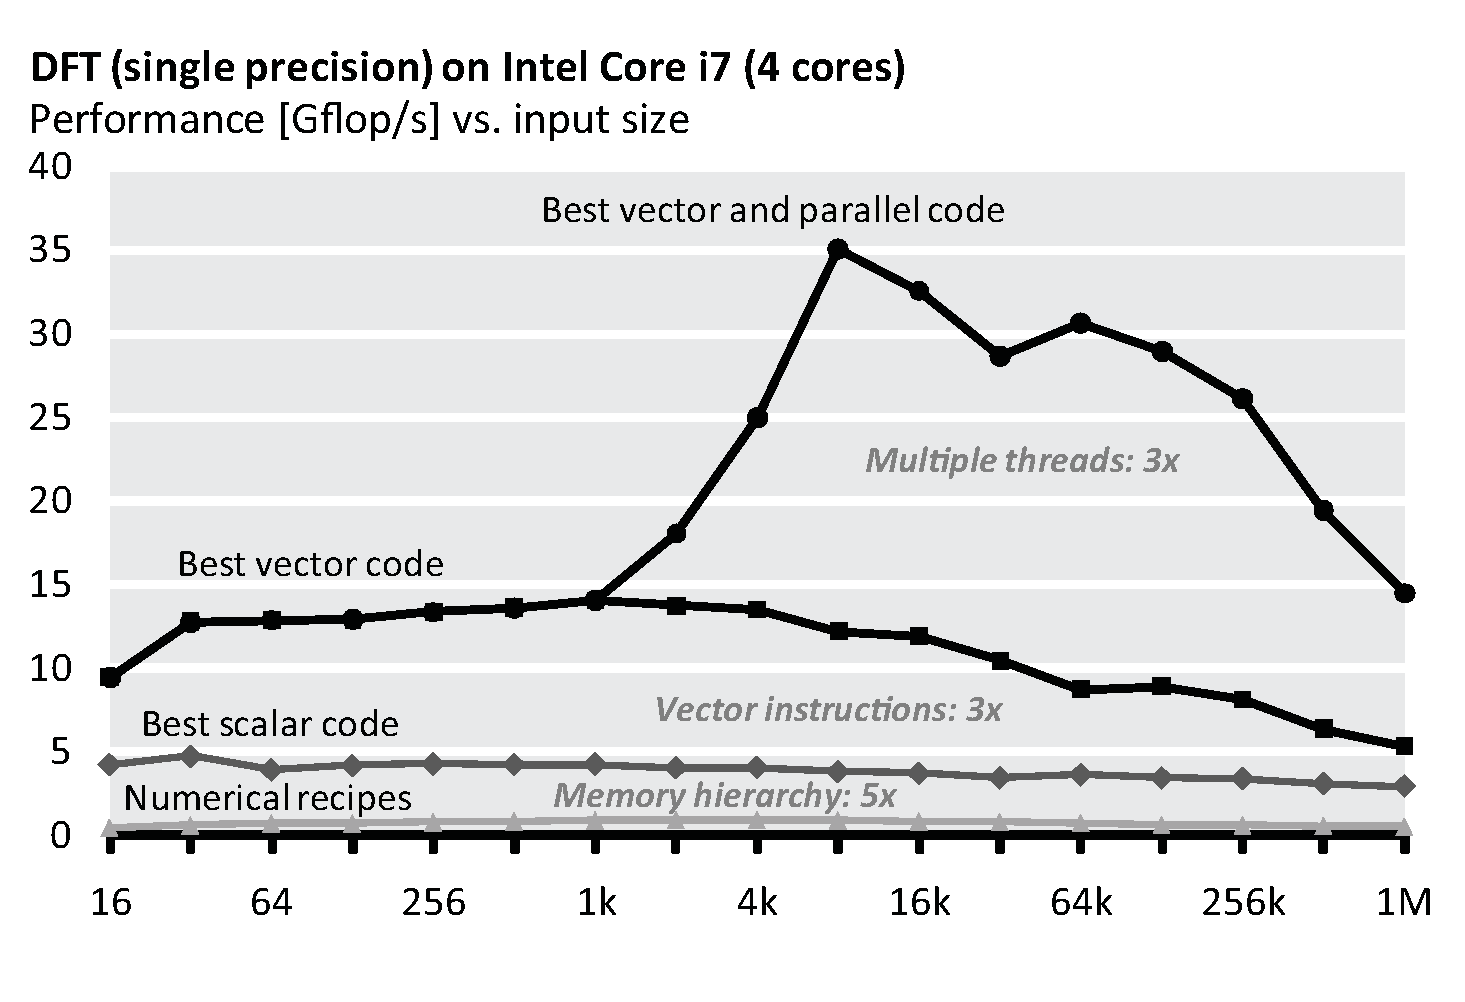
\includegraphics[scale=0.33]{dft-performance.eps}
  \caption{Performance of four single precision implementations of the
  discrete Fourier transform. The operations count is roughly the
  same. The labels in this plot are maybe a little bit too small.\label{fftperf}}
\end{figure}

\section{Conclusions}

Here you need to summarize what you did and why this is
important. {\em Do not take the abstract} and put it in the past
tense. Remember, now the reader has (hopefully) read the report, so it
is a very different situation from the abstract. Try to highlight
important results and say the things you really want to get across
such as high-level statements (e.g., we believe that .... is the right
approach to .... Even though we only considered x, the
.... technique should be applicable ....) You can also formulate next
steps if you want. Be brief. After the conclusions there are only the references.

\section{Further comments}

Here we provide some further tips.

\mypar{Further general guidelines}

\begin{itemize}
\item For short papers, to save space, I use paragraph titles instead of
subsections, as shown in the introduction.

\item It is generally a good idea to break sections into such smaller
units for readability and since it helps you to (visually) structure the story.

\item The above section titles should be adapted to more precisely
reflect what you do.

\item Each section should be started with a very
short summary of what the reader can expect in this section. Nothing
more awkward as when the story starts and one does not know what the
direction is or the goal.

\item Make sure you define every acronym you use, no matter how
convinced you are the reader knows it.

\item Always spell-check before you submit (to us in this case).

\item Be picky. When writing a paper you should always strive for very
high quality. Many people may read it and the quality makes a big difference.
In this class, the quality is part of the grade.

\item Books helping you to write better: \cite{Higham:98} and \cite{Strunk:00}.

\item Conversion to pdf (latex users only): 

dvips -o conference.ps -t letter -Ppdf -G0 conference.dvi

and then

ps2pdf conference.ps
\end{itemize}

\mypar{Graphics} For plots that are not images {\em never} generate the bitmap formats
jpeg, gif, bmp, tif. Use eps, which means encapsulate postscript. It is
scalable since it is a vector graphic description of your graph. E.g.,
from Matlab, you can export to eps.

The format pdf is also fine for plots (you need pdflatex then), but only if the plot was never before in the format 
jpeg, gif, bmp, tif.


% References should be produced using the bibtex program from suitable
% BiBTeX files (here: bibl_conf). The IEEEbib.bst bibliography
% style file from IEEE produces unsorted bibliography list.
% -------------------------------------------------------------------------
\bibliographystyle{IEEEbib}
\bibliography{bibl_conf}

\end{document}

